\section{Assignment 12}

\subsection{Implement the impedance control in the operational space}

\begin{figure}[H]
\centering
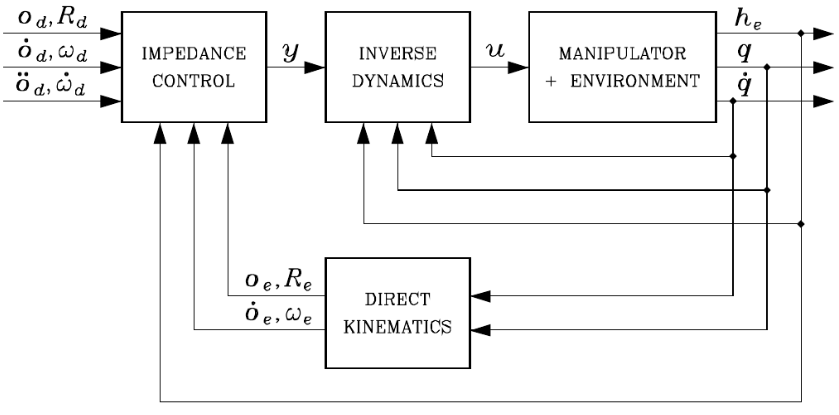
\includegraphics[keepaspectratio,width=.5\textwidth]{impedance_arch}
\caption{Impedance control in operational space architecture}
\end{figure}

The architecture implements the following stabilizing linear control law:

\begin{equation*}
y = J_A^{-1}(q)M_d^{-1}(K_D\dot{\tilde x} + K_P\tilde x - M_d\dot J_A(q,\dot q)\dot q - M_db(\tilde x,R_d,\dot o_d,\omega_d)-h_e^d)
\end{equation*}

The architecture is based on the definition of a mechanical impedance defined by an equivalent mass matrix $M_d$, an equivalent damping matrix $K_D$ and an equivalent stiffness matrix $K_P$. The mechanical impedance is independent from the configuration of the robot.

The architecture is modelled in SIMULINK as follows:

\begin{figure}[H]
\centering
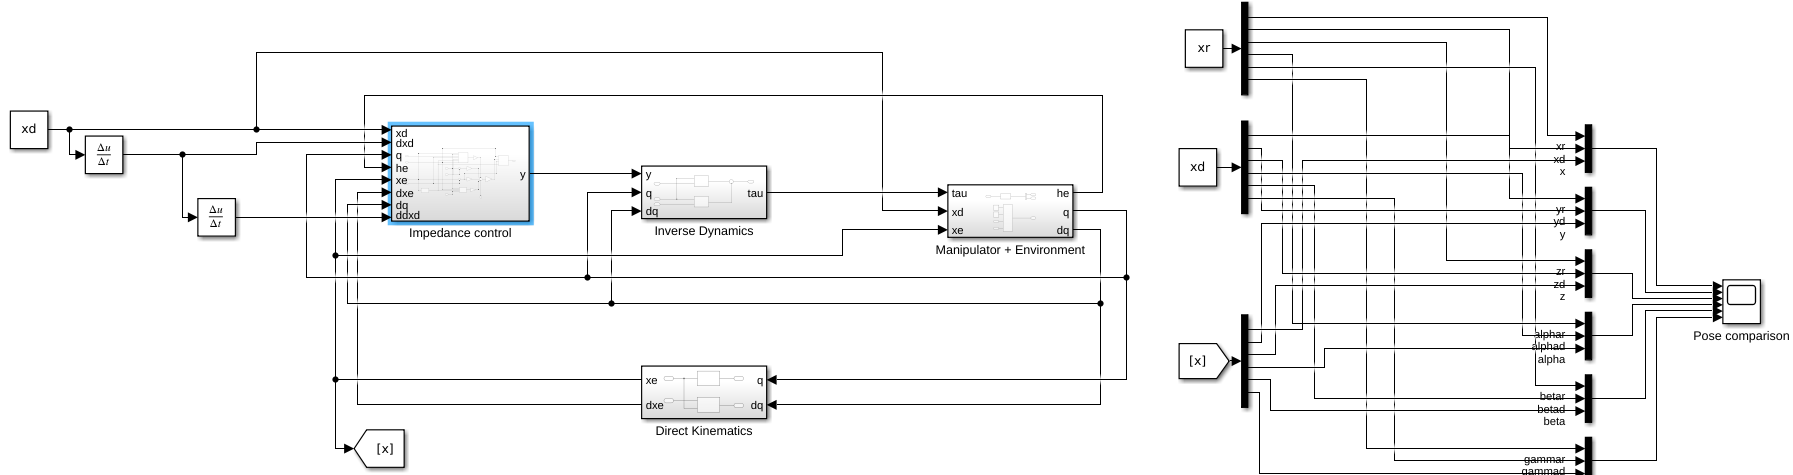
\includegraphics[keepaspectratio,width=\textwidth]{impedance_sim}
\caption{Impedance control in operational space SIMULINK model}
\end{figure}

To test the architecture, the manipulator was moved to $x_0=k(\begin{bmatrix}
0&-0.3&0
\end{bmatrix})$, with a desired position of $x_d=k(\begin{bmatrix}
0&-0.2&0
\end{bmatrix})$ and the environment placed at $x_e=k(\begin{bmatrix}
0&-0.1&0
\end{bmatrix})$. This was done to simplify the architecture, allowing for contact only in the $y$ direction. The mechanical impedance was defined with $M_d=\begin{bmatrix}
0.3 & 1 & 0.3 & 0.3 & 0.3 & 0.3
\end{bmatrix}$, $K_D=\begin{bmatrix}
30 & 25 & 30 & 30 & 30 & 30
\end{bmatrix}$ and $K_P=\begin{bmatrix}
50 & 75 & 50 & 50 & 50 & 50
\end{bmatrix}$.

\newpage

\begin{figure}[H]
\centering
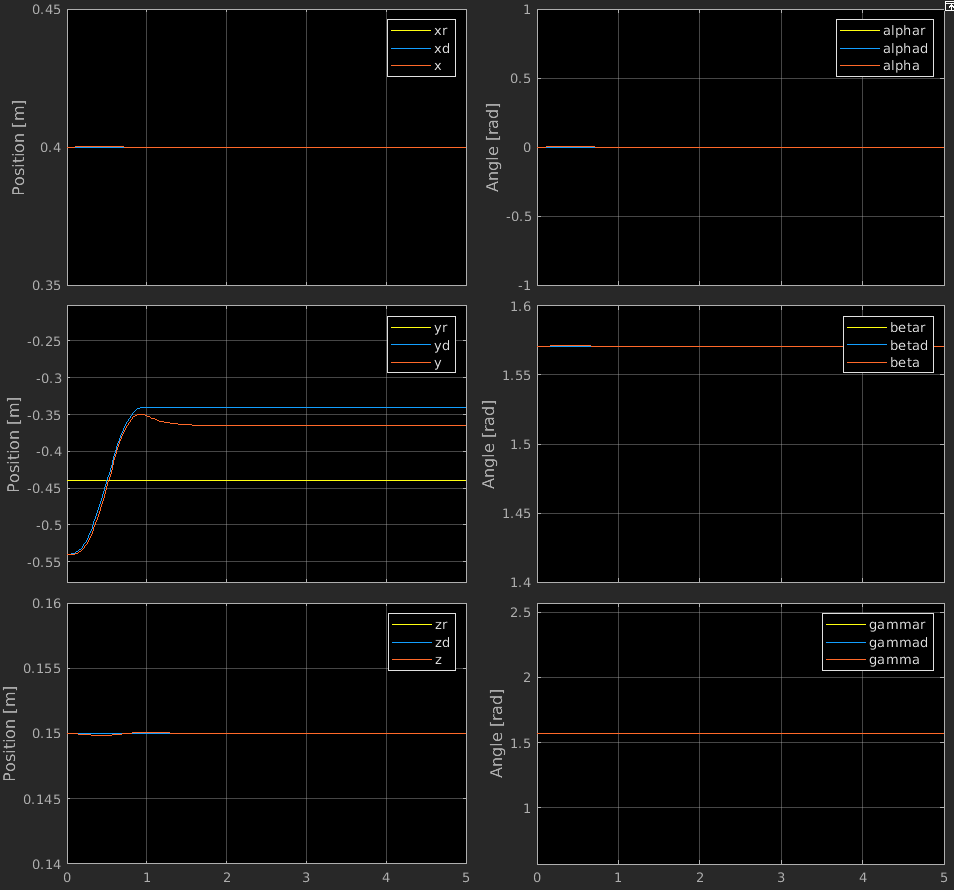
\includegraphics[keepaspectratio,width=\textwidth]{impedance_1}
\caption{Impedance control}
\end{figure}